\chapter{Jefferson Lab and CLAS}

\section{Background}
The Thomas Jefferson National Accelerator facility, more commonly known as Jefferson Lab or JLab, is a U.S. national laboratory located in Newport News, Virginia, U.S. Its physics program is designed to probe the structure of hadrons to better understand the fundamental properties of nuclear matter. 

\begin{figure}
	\centering
	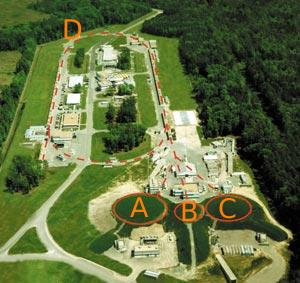
\includegraphics[width=0.6\textwidth]{ImgChap1/jlab1}
	\caption{Photograph of JLAB}
	\label{JLABAirial}
\end{figure}

The research program at the laboratory is based around the Continuous Electron Beam Facility (CEBAF) a superconducting radiofrequency based accelerator based around two anti-parallel linacs linked by 9 recirculation beam lines that allow up to 5 passes through the system. The facility produces a continuous wave electron beam with energies exceeding 6 GeV and luminosities of $< 10^{38} cm^{-2}s^{-1}$. For further information on CEBAF see \cite{leemann2001continuous}.

\textbf{Some further detail on the beamline.}

\begin{figure}
\centering
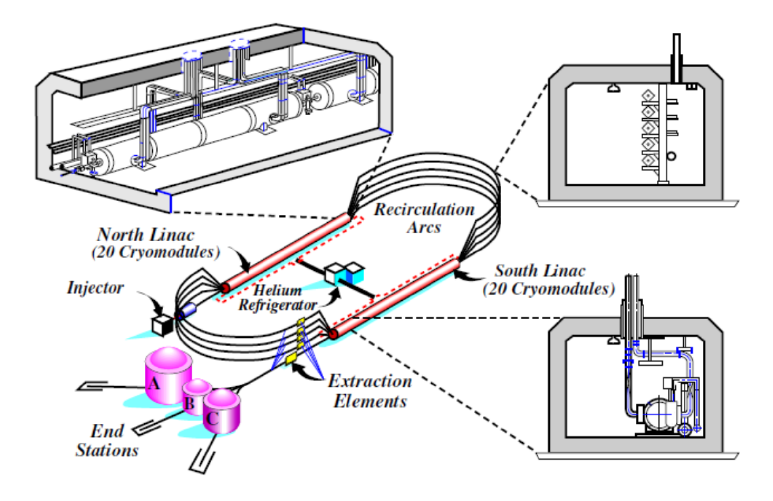
\includegraphics[width=0.6\textwidth]{ImgChap1/CEBAF1}
\caption{A schematic layout of CEBAF.}
\label{CEBAF}
\end{figure}

The primary beam is separable and the facility is capable of delivering beams to 3 different experimental halls for simultaneous experiments. Each of the experimental halls in CLAS is designed to be complimentary providing different facilities address a broad range of physics goals.

\begin{figure}
	\centering
	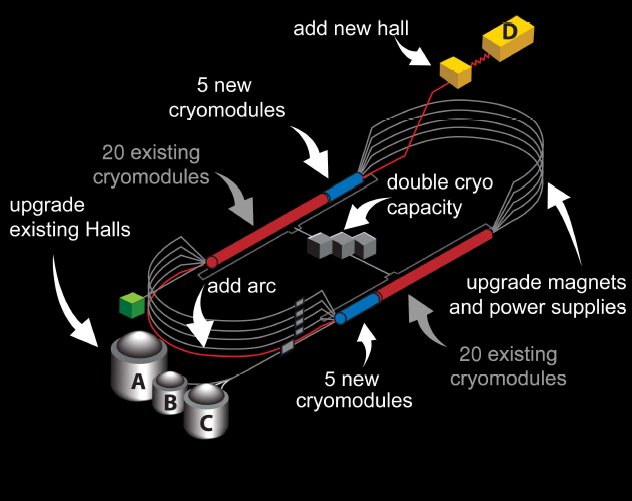
\includegraphics[width=0.6\textwidth]{ImgChap1/CEBAF}
	\caption{A schematic layout of CEBAF after the 12 GeV upgrade is completed.}
	\label{CEBAF12}
\end{figure}

In June 2010 construction began on an $\$338$ million upgrade to Jefferson Lab upgrading the beamline to a maximum energy of 12 GeV and adding a fourth experimental hall to the facility (Hall D). The investment also includes upgrades for the existing experiments in halls A, B and C. Presenting both new challenges and opportunities for the working groups. 

Hall A is equipped with a pair of identical high resolution spectrometers capable to processing luminosities $< 10^{38} cm^{-2}s^{-1}$. Its research program includes work on nucleon structure functions and nucleon form factors. \cite{alcorn2004basic}

Hall B houses the CEBAF Large Acceptance Spectrometer a wide acceptance detector designed to study electro and photo induced nuclear and hadronic reactions. The detector required efficient detection of both charged and neutral reactions products to be able to study exclusive reactions. \cite{mecking2003cebaf}

Hall C main focus is a pair of \textbf{Missing Detail for Hall C}

Hall D \cite{qiang2015detector}


The work presented in this thesis is focussed around physics undertaken in Hall B at JLab and the CLAS detector situated within it.

\section{CLAS}
CLAS is a wide acceptance detector utilising a toroidal magnetic field that is situated in Hall B at JLab. Its primary design aims are to measure the momentum of charged particles with high resolution, covering a wide geometric area up to large angles in the laboratory and keep a magnetic field free region around the target, to allow the use of dynamically polarised targets.

\begin{figure}
	\centering
	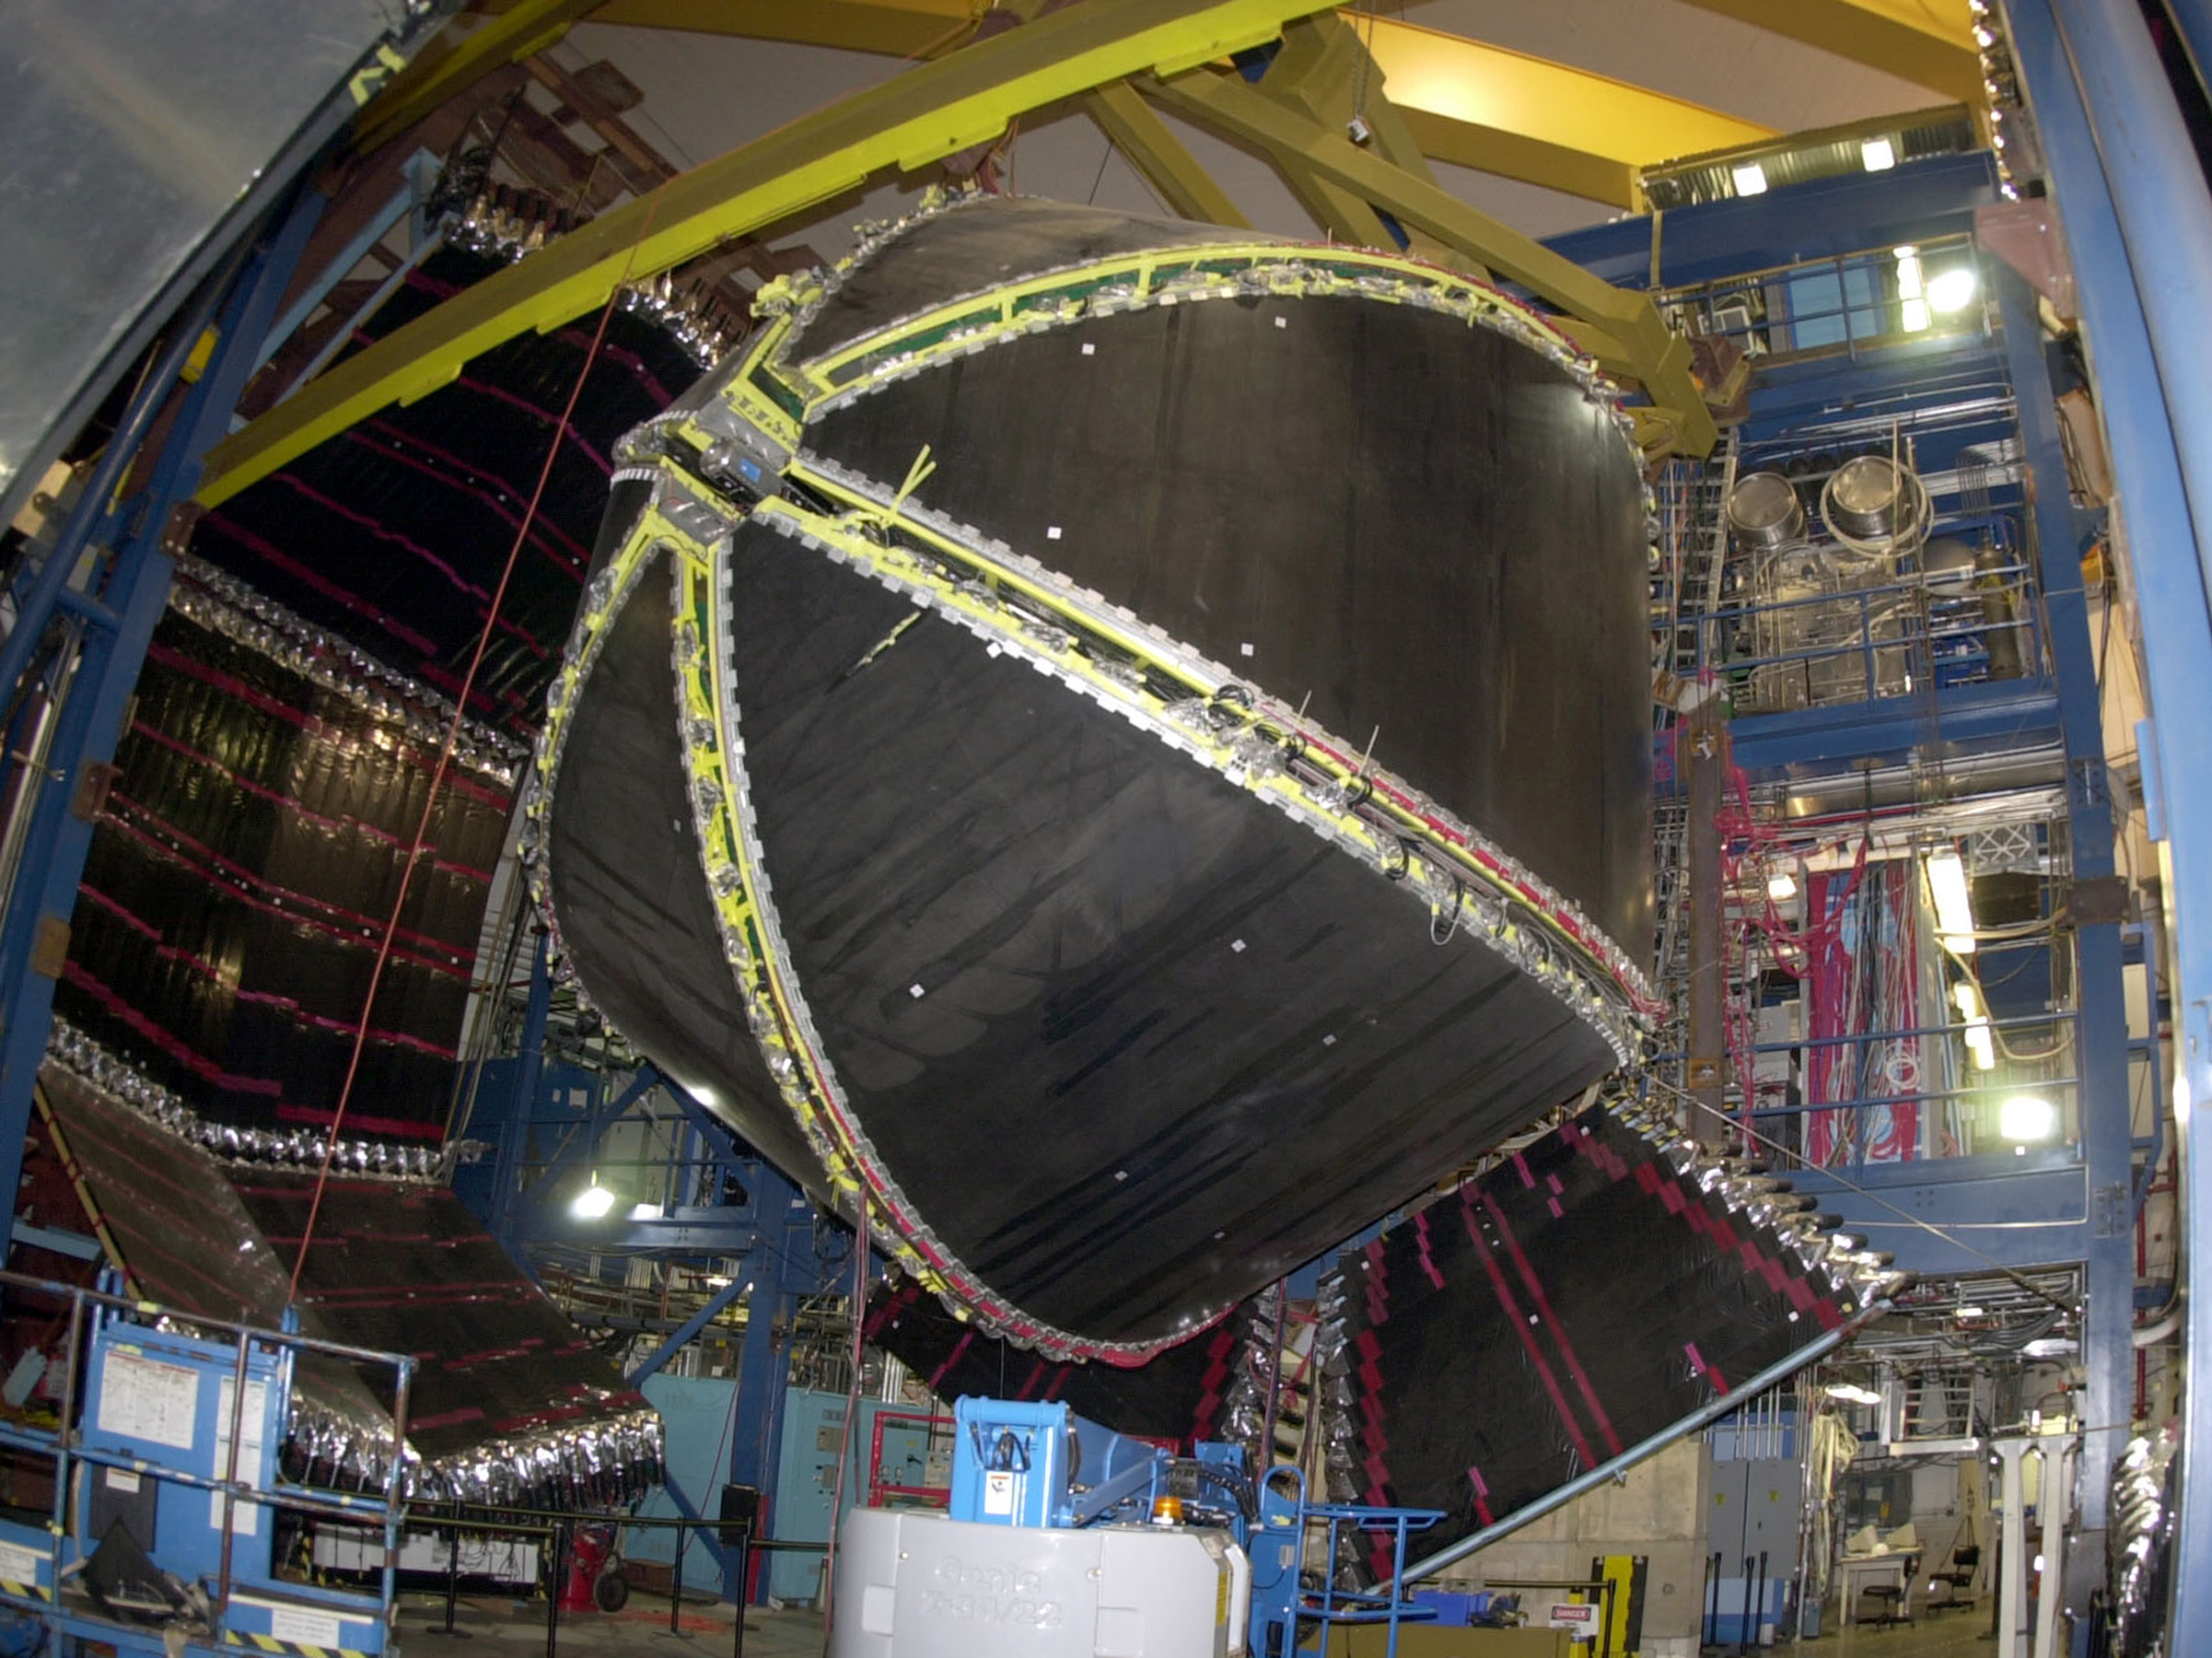
\includegraphics[width=0.6\textwidth]{ImgChap1/CLASPhoto}
	\caption{Photograph of the CLAS detector.}
	\label{CLASPhoto}
\end{figure}

The magnetic field in CLAS is generated by 6 superconducting coils that are arranged symmetrically around the beamline at $60\textdegree$ intervals. These produce a field primarily orientated in the $\theta$-direction perpendicular to the beamline.

\begin{figure}
	\centering
	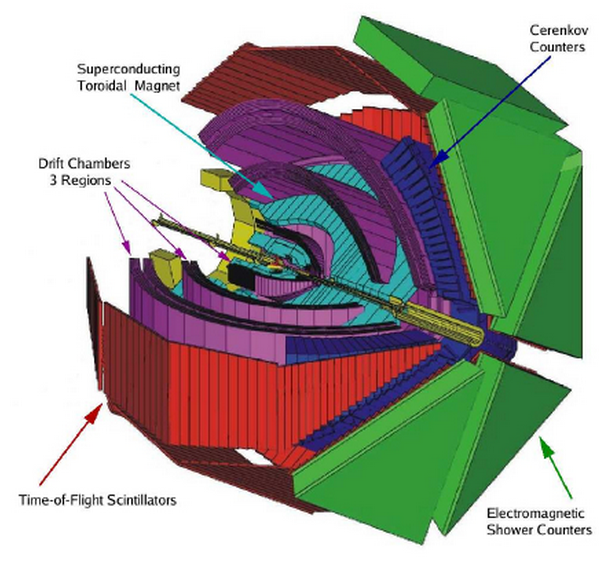
\includegraphics[width=0.6\textwidth]{ImgChap1/CLAS1}
	\caption{Schematic picture of CLAS with the different subsystems highlighted in colour. \textbf{CITATION}}
	\label{CLASDiagram}
\end{figure}

The detector makes use of drift chambers to determine the trajectories of particles. \cite{mestayer2000clas} Gas cherenkov detectors to differentiate between electrons and pions in the detector. \cite{adams2001clas} Scintillation counters for measuring the ToF of particles through the detector. \cite{smith1999time} Finally two types of electromagnetic calorimeters to determine the characteristics of the particle showers and measure the energy deposited. Forward \cite{amarian2001clas} and large angle \cite{anghinolfi2000response}.

The design means the detector is essentially composed of 6 independent magnetic spectrometers working in unison. With each sharing a common target, trigger and readout mechanism. The detector is designed to be suitable for both electron and photon beam experiments, however adjustments are made for different beam conditions. When are electron beam is in use, a 'mini-torus' is added around the target to shield the inner most drift chambers from electrons produced through M\o{}ller scattering in the target. For photon beams a start counter is added inside in the inner drift chambers to provide precision timing for reactions. \cite{taylor2001clas}


%CLAS paper \cite{mecking2003cebaf}
%
%Drift chambers for to determine the trajectories of charged particles \cite{mestayer2000clas}
%
%Gas cherenkov detectors for electron indentification \cite{adams2001clas}
%
%scintillator counters for measuring time of flight \cite{smith1999time}
%
%electromagnetic calorimeters to detect showering particles.
%Forward \cite{amarian2001clas}
%large angle electronmagnetic calorimeter \cite{anghinolfi2000response}

%Detector suitable for both electron and photon beam experiments, however a adjustment is made for the different beam conditions.
%For an electron beam a 'mini-torus' is added around the target to shield the inner most drift chambers from electrons produced through M\o{}ller scattering in the target.
%
%Start counter used for tagged-bremsstrahlung experiments \cite{taylor2001clas}

\subsection{Tagged-Bremsstrahlung}

In CLAS photon beams are produced through by passing the CEBAF electron beam through a thin target (the "radiator") positioned just upstream of a magnetic spectrometer (the "tagger") The system uses electron bremsstrahlung reactions during which an incident electron of energy $E_{0}$ is scattered by the electromagnetic field of a nucleus, causing an energetic photon to be released. The energy transferred to the nucleus during the reaction is negligibly small, so the energy conservation reaction can be written as

\begin{equation}
E_{\gamma} = E_{0} - E_{e}
\end{equation}


Where $E_{\gamma}$ is the energy of the photon and $E_{e}$ is the energy of the post-reaction electron. From this if the energy of the electron beam is known. Then the energy of the photon can be resolved from determining the energy of the scattered electron in a magnetic spectrometer. \cite{sober2000bremsstrahlung}

\begin{figure}
	\centering
	\includegraphics[width=0.9\textwidth]{ImgChap1/Brem1improved}
	\caption{Diagram of the bremsstrahlung production mechanism and the spread of electron energies measurement which allow the energy of the photon beam to be resolved. \cite{sober2000bremsstrahlung}}
	\label{CLASbrem}
\end{figure}

The production angle of the photon is dependent on beam energy and at energies great than a few MeV the photon and electron emerge at angles little deviated from the beam direction. The scatter angle of the photon is also dependent on the rest of the electron $m_{e}$ and follows the relation

\begin{equation}
\theta_{\gamma} = mc^{2} / E_{0}
\end{equation}


The corresponding scatter angle of the electron is given by

\begin{equation}
\theta_{e} = \theta_{\gamma}E_{\gamma} / E_{e}
\end{equation}

At the energies utilised at Jefferson Lab, both of these angles are of the order of 1 mr or smaller. To a first approximation it can be taken that the photon and electron travel in the same direction as the original beam. The produced photons pass through the field produced by the tagger magnet continue on towards the beam target. These are further constrained by a series of collimators placed just downstream of the tagger. Details of this mechanics and the structure of the tagger are shown in Figures \ref{CLASbrem} and \ref{CLASbrem1}.

The strength of the tagger magnet is adjusted depending on the beam energy to ensure those electrons that do not radiate will follow an arc directly into a shielded beam dump. Those that do will follow a tighter arc with a spread dependent on the percentage of incident energy transferred to the photon and the strength of the tagger field. A flat plane segmented scintillator hodoscope is positioned to cover the arc of electrons covering an energy range of $20\%$ to $95\%$ of the electron beam energy. This requires sufficient segmentation to provide adequate energy resolution and fast enough timing resolution to be able to separate the 2 ns separated beam bunches. In order to minimise the effects of re-scattering the electrons are pass through a thin exit window just after scatting into a vacuum chamber until they reach the scintillators. \cite{sober2000bremsstrahlung}


\begin{figure}
	\centering
	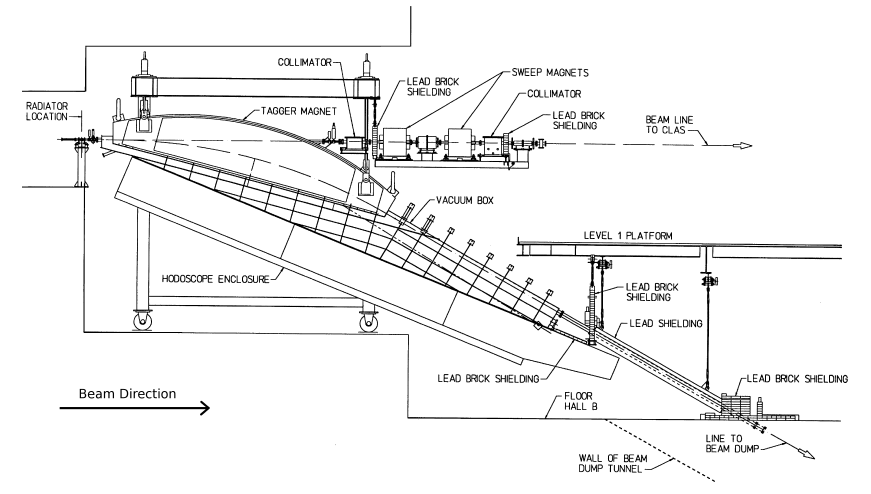
\includegraphics[width=0.9\textwidth]{ImgChap1/BremFac}
	\caption{Diagram of the contruction of the bremsstrahlung production mechanism. In particular highlighting, the radiator, vacuum chamber and collimator positioning. \cite{sober2000bremsstrahlung}}
	\label{CLASbrem1}
\end{figure}


\subsection{Detectors Systems}


\subsubsection{Torus Magnet} \cite{street1996final} \cite{o1989superconducting}

The magnetic field required for momentum analysis within CLAS is generated by 6 superconducting coils arranged in a toroidal shape around the beamline. The combined arrangement forms a system of $\sim$5m in length and and 5m in diameter. The symmetric design produces a magnetic field which is primarily focused in the $\phi$-direction, with some deviation close to each of the magnetic coils. Whilst also maintaining a largely field free region in the centre of the detector region allowing for the operation of a polarized target. Figure \ref{MagneticFields1} shows the vectors of the magnetic field from the viewpoint along the beamline. The length of the vectors are proportional to the strength of the magnetic field at each point.

\begin{figure}
	\centering
	\includegraphics[width=0.6\textwidth]{ImgChap1/meson2}
	\caption{Torus magnets.}
	\label{CLAStorus}
\end{figure}

\begin{figure}
	\centering
	\includegraphics[width=0.6\textwidth]{ImgChap1/mag}
	\caption{Torus magnets.}
	\label{MagneticFields1}
\end{figure}

Each of these coils that form the system is kidney shaped producing a field which more strongly effects particles scattered at forward angles (with typically higher momentum) with more limited effects at wider scatter angles. At the maximum design current of 3860 A, the integral of the field strength of forward angles reaches 2.5 T at forward angles dropping to 0.6 T at a scatter angle of $90\deg$. Field lines of equal strength are shown in Figure \ref{MagneticFields2} from a perspective between two of the superconducting coils.

\begin{figure}
	\centering
	\includegraphics[width=0.6\textwidth]{ImgChap1/mag1}
	\caption{Torus magnets.}
	\label{MagneticFields2}
\end{figure}

\subsubsection{Drift Chambers} \cite{mestayer2000clas} \cite{carman1998region} \cite{qin1998prototype}

The magnetic field generated by the coils bends charged particles either away or towards the beamline, with minimal effect in the azimuthal direction. The particles trajectories by a 6-way symmetric arrangement of 18 drift chambers split into 3 'regions' (R1, R2 and R3) matching the natural geometry arising from the arrangement of the 6 superconducting coils. The R1 drift chambers are positioned just outside the target area in a region of low magnetic field. The R2 drift chambers are positioned between the magnetic coils in an area high field near the point of maximum sagitta for the charged particles. The R3 chambers are positioned outside the magnetic coils in a region of lower magnetic field. Their relative positions and orientations are shown in Figure \ref{CLASdrift}.

\begin{figure}
	\centering
	\includegraphics[width=0.6\textwidth]{ImgChap1/meson2}
	\caption{Drift Chambers positions.}
	\label{CLASdrift}
\end{figure}

For optimal coverage and maximum sensitivity to the radius of curvature, the drift chambers are positioned between each of the magnetic coils at $60\deg$ intervals approximately perpendicular to the bend plane. The chambers fill the wedge shape detector volumes with field and sensing wires spaced to form a series 'layers' of concentric partial circles with wires in each layer positioned half a wire diameter along from the next. Forming an arrangement similar in geometry to hexagonal close packing throughout the detector volume. This is shown clearly in Figure \ref{CLASdriftwires}. The size of the hexagonal structures increases in proportion to the distance from the centre of the detector.

\begin{figure}
	\centering
	\includegraphics[width=0.6\textwidth]{ImgChap1/meson2}
	\caption{Drift Chambers positions.}
	\label{CLASdriftwires}
\end{figure}

For improved tracking and azimuthal information, each drift chamber is split into two 'superlayers', one axial to the magnetic field and the other with a $6\deg$ tilt to provide stereo azimuthal information. An exception to this is R1, due to space limitations it has only a single axial layer. 

For safety and detector longevity reasons the wires chambers are filled with a $88\%-12\%$ mix of argon and $CO_{2}$ which is controlled by an active feedback systems which maintains constant system conditions adjusting for any changes in the surrounding environment. 

The detector resolution is dependent on single wire resolution along with uncertainties from multiple scattering in the material, the true value of the magnetic field strength and misalignments in the geometry of the detector system. Single wire resolution is dependent on where within the cell a track passes. With increasing uncertainty when close to either the sensing or field wires and improved resolution towards the middle of each cell. This is due to ion-pair production near the sensing wire and divergence of the magnetic field and time walk affects near the field wires in a cell. The resolution for a track pathing in the mid region of a cell is 200-250 $\mu$m. With a whole cell average of $\sim$ 310, 315 and 380 $\mu$m for R1, R2 and R3 respectively. \cite{mecking2003cebaf} 


\subsubsection{Cerenkov Counters}

\cite{adams2001clas}

The Cerenkov counters serve the dual purpose of differentiating between electrons and pions and providing a trigger on electrons. They are designed to maximise the solid angle coverage in each of the six sectors up to $\theta = 45$ whilst using the minimum amount of material (To limit its effect on energy resolution). This is achieved by placing the Photomultiplier tubes and light collection cones in regions in $\phi$ which are already shadowed by the structure of the toroidal magnets and covering as much of the solid angle as possible with mirrors. Figure \ref{CLAScerenkov} shows the layout of one of the Cerenkov detectors.

\begin{figure}
	\centering
	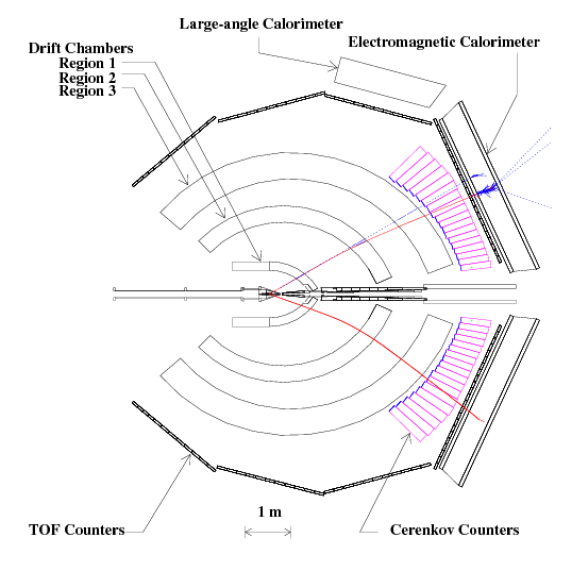
\includegraphics[width=0.6\textwidth]{ImgChap1/CLAS2}
	\caption{Cerenkov layout, get a better picture, that shows the structure of the Cerenkov.}
	\label{CLAScerenkov}
\end{figure}

Coverage of $\theta$ in each of the six sectors of CLAS is divided into 18 regions and each of these was further subdivided into two modules bisecting the centre of each of the 6 sectors. Resulting in a total of 12 identical subsectors about the $\phi$-axis for each of the 18 sections in $\theta$ for a total of 216 Cerenkov modules. \cite{adams2001clas}

\subsubsection{Time of Flight Counters}

This detector system covers the azimuthal angle $\phi$ between $8\deg$ and $142\deg$ and works in conjunction with the start counter, when using photon beams, to determine the time of flight of particles (ToF) within CLAS. Particles propagating radially outwards from the target will reach the ToF counters after passing through the drift chambers and at forward angles also the Cerenkov counters.

The detectors are composed of Bicron-408, a fast responding plastic scintillator, in sections 5.08cm thick, designed to produce signals of large amplitude from minimum ionising particles passing through the detector. Each scintillator block is positioned to be perpendicular to the mean propagation direction of reaction products, covering $\sim 1.5 \deg \theta$. The forward angle counters ($\theta < 45$) are 15 cm wide, and those at wider scattering angles are 22 cm wide in the $\Delta\theta$ direction. The forward angle counters are between 32 and 376 cm in length and the wide angle detectors are 371 to 445 cm in length, with timing resolutions of between $\sim 90-160 ps$ For scintillators of these dimensions the dominant contribution to timing resolution is the varying path length of photons produced in the materials on their way to the PMTs. The spread of these is shown in Figure \ref{CLAStof} For further information on the ToF counters see \cite{smith1999time}.

\begin{figure}
	\centering
	\includegraphics[width=0.6\textwidth]{ImgChap1/meson2}
	\caption{Spread of timing resolution for the ToF detectors.}
	\label{CLAStof}
\end{figure}

\subsubsection{Electromagnetic Calorimeters}

CLAS utilises a Forward Electromagnetic Calorimeter (FC) that covers its full acceptance range in $\phi$ and up to $\theta$ = $45\deg$ and an additional Large Angle Electromagnetic Calorimeter (LAC) that covers 2 of 6 sectors of CLAS in the range $\theta$ = $45\deg-75\deg$. This section will focus on the main FC but the LAC has a similar design and additional detail can be found in \cite{anghinolfi2000response}. The main functions of the FC detector system are identification and triggering of electrons above 0.5 GeV, detection of photons above 0.2 GeV, (For reconstruction of $\pi^{0}$ and $\eta$) and neutron detection. It covers a range up to $\theta$ = $45\deg$ and is constructed from alternating layers of lead and scintillator in a 0.24 ratio. 

The system is split into 6 sectors positioned between the coils of the torus forming a shape approximating an equilateral triangle. There are 39 layers in the detector system, comprised from 10mm of scintillator followed by 2.4 mm of lead. These layers follow a "projective" geometry directed towards the nominal target position, with each subsequent layer progressing radially outwards, covering a linearly increasing area.  Each layer is composed of 36 strips rotated through $120\deg$ with respect to the previous layer and readout at one of the three edges of each sector. Depending on their orientation the 39 layers are split into 3 groups (U,V and W) to provide stereo information on the location of the energy deposited. These groups are further subdivided into an inner (5 layers) and outer (8 layers) stack for greater longitudinal information to improve hadron and electron separation.

\begin{figure}
	\centering
	\includegraphics[width=0.6\textwidth]{ImgChap1/meson2}
	\caption{Picture of the forward EC and the LAC.}
	\label{CLASForwardEC}
\end{figure}

Hit reconstruction requires a hit in U,V and W layers of the detector in either the inner or outer potions of a sector. Positions are calculated by reconstructing the intersection points of strips triggered above threshold, weighting appropriately for the timing an energy response depending on the position of the hit in the detector system. Hits recorded within 10cm of the edge of the detector volume are discarded to ensure the full electromagnetic shower is contained within the sensitive region of the detector. Using electrons as an example for the performance of the detector; for those above 3 GeV the sampling fraction of the system is $\sim 0.3$. Below this the rate decreases falling to 0.25 for electrons of 0.5 GeV. For electron showers that deposit more than 0.5 GeV in the scintillator the rms position resolution is $\sim 2.3 cm$. Finally, the timing resolution for electrons averages 200 ps across the detector system. For further information on the forward electromagnetic calorimeter see \cite{amarian2001clas}.

\subsubsection{Start Counter}

%General overview of the subsystems of clas
%Calorimeters
%Drift Chambers
%Start Counter
%Magnets
%etc

\section{The upgrade to CLAS12}
System upgrades
System additions like the forward tagger covering the forward angle of the beamline.

What the upgrade will mean for the physics programs in Hall B.